\chapter{Teori}
%
\begin{figure*}[htpb]
    \centering
    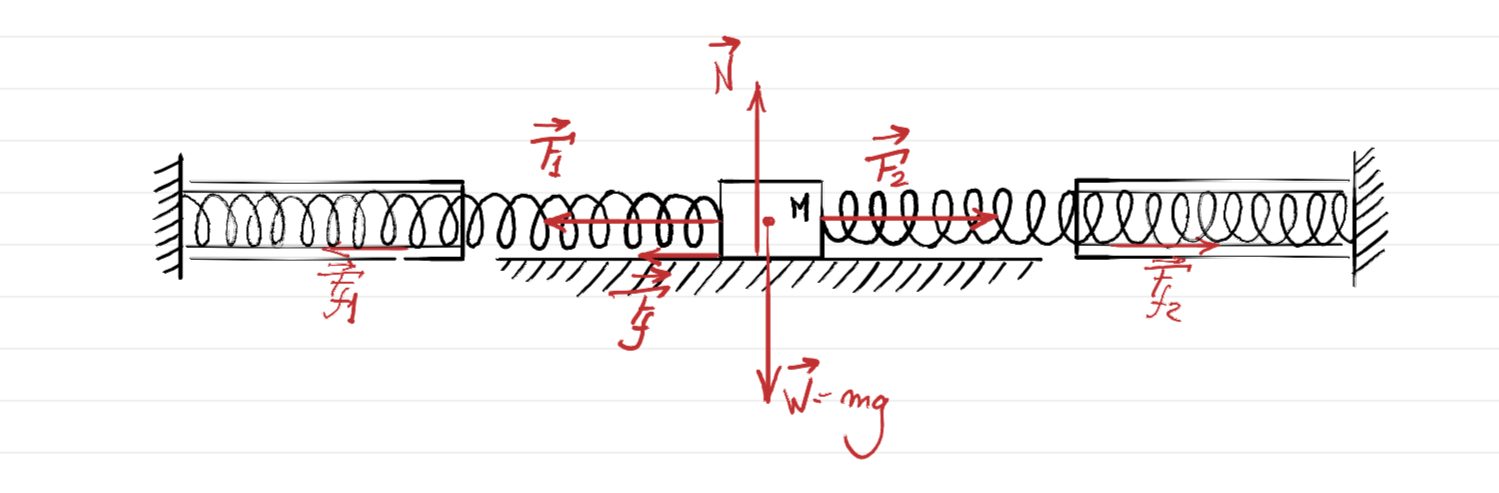
\includegraphics[width=0.8\linewidth,origin=c]{figures/systemskitse.png}
    \caption{Skitse af systemet (kraft betegnelser stemmer ikke overens med resten af opgaven)}
    \label{fig:skitse}
\end{figure*}
%
Betragt et system af en masse forbundet til 2 fjedrer, en i hver ende, der hver er forbundet til en væg, med fjeder konstanterne $k_1$ og $k_2$. 
Massen er placeret på en vandret overflade med friktionskoefficienter $\mu_s$ og $\mu_k$. 
Fjedrernes bevægelse har også friktion med en anden friktionskoefficient $\delta_s$ og $\delta_k$ \cite{YF}.
Normalkraften mellem overfladen og massen, samt mellem fjeder og dens overflade er ikke nødvendigvis den samme, og betegnes derfor seperat med $n_1$ og $n_2$.
Vi betegner massen af det samlede oscillerende legeme med $m$. 

Newtons anden lov for systemet afhænger af hvilken retning vi bevæger os i. 
Vi må derfor opstille Newtons anden lov 2 gange, nemlig for tilfældet med bevægelse i positiv og negativ x-retningen. 
Vi opstiller vores koordinatsystem sådan at 0 punktet ligger der hvor de 2 fjedrer trækker lige meget, altså fjeder systemets ligevægtsposition. Vi indser også at de 2 fjedrer tilsammen fungerer som en samlet fjeder med fjederkonstant $k = k_1 + k_2$.
\begin{align*}
    \Sigma F_{x_+} = -kx - \mu_k n_1 - \delta_k n_2 = ma\\
    \Sigma F_{x_-} = -kx + \mu_k n_1 + \delta_k n_2 = ma
\end{align*}
Hvis vi samler de 2 gnidningskrafter i en konstant $f_k$, får vi følgende differentialligninger (skrevet som en differentialligning med $\pm$ for overskuelighed)
\begin{equation}
    \odv[order=2]{x}{t} + \frac{k}{m}x = \pm \frac{f_k}{m}
\end{equation}
Dette er en inhomogen lineær anden ordens differentialligning \cite{calc}, hvor samtlige løsninger kan findes 
som den fuldstændige løsning til den homogene ligning plus en partikulær løsning til den inhomogene.
Vi kan genkende den homogene differentialligning (hvor konstanten er 0), som blot værende differentialligningen for en harmonisk oscillator, 
og vi ved derfor at den fuldstændige løsning er $x(t) = A\sin\omega t + B\cos\omega t$ hvor $\omega = \frac{k}{m}$. Vi mangler derfor kun at finde en partikulær løsing til den inhomogene.
Her gætter jeg på løsningen $x(t) = \pm \frac{f_k}{k}$, da man indser
\[
     \odv[order=2]{\frac{f_k}{k}}{t} + \frac{k}{m}(\pm\frac{f_k}{k}) = \pm \frac{f_k}{m}
\]
Den fuldstændige løsning til de inhomogene differentialligninger bliver altså
\begin{equation}
    x(t) = A\sin\omega t + B\cos\omega t \pm \frac{f_k}{k}
\end{equation}
Nu bliver det dog besværligt. Eftersom at bevægelsesligningerne ændrer sig hver gang bevægelsesretningen skifter, 
bliver vi nødt til rekursivt at finde startbetingelserne hver gang bevægelsesretningen skifter.
Start betingelserne vil hver gang være en start amplitude $x(0) = x_n$ og en start hastighed $x'(0) = 0$. Denne er altid nul når bevægelsesretningen skifter, da dette sker i en fuldt udstrakt position hvor alt den kinetiske energi er lagret i fjedrerne.

Hvis vi starter vores bevægelse i amplitude $-x_0$, bliver bevægelsesbetingelserne efter indsættelse i (2)
\begin{align*}
    x(0) &= B - \frac{f_k}{k} = -x_0 \implies B = -x_0 + \frac{f_k}{k} \\
    x'(0) &= \omega A = 0 \implies A = 0 \\
    \shortintertext{$A$ og $B$ indsættes i (2)}
    x(t) &= (-x_0 + \frac{f_k}{k})\cos \omega t - \frac{f_k}{k}
\end{align*}
Bemærk at konstant ledet har negativt fortegn da vi bevæger os i den positive x-retning, da startamplituden er negativ.
Som sagt beskriver denne forskrift kun bevægelsen indtil at den ændrer bevægelsesretning. 
Hvis vi vil finde forskiften for bevægelsen efterfølgende, bliver vi nødt til at vide hvad startamplituden er for den nye bevægelse.
Den kan vi nemt finde som anden gang et hastigheden er 0.
\[
x'(t) = \omega(x_0 - \frac{f_k}{k})\sin \omega t = 0
\]
Da de andre termer ikke er 0, og $t = 0$ ikke er en valid løsning, da det er hvor bevægelses starter, må det være næste nulpunkt, nemlig $t = \frac{\pi}{\omega}$. 
Læg mærke til at perioden er uafhængig af amplituden.
Indsætter vi den tid i vores udtryk for $x(t)$, får vi 
\[
x(\frac{\pi}{\omega}) = x_0 - \frac{2f_k}{k} \equiv x_1
\]
Anvender vi den amplitude som startbetingelser for bevægelsen tilbage i negativ x-retningen, får vi bevægelsesligningen:
\[
x(t) = (x_1 - \frac{f_k}{k})\cos \omega t + \frac{f_k}{k}
\]
Hvilket leder til at den næste start amplitude bliver 
\[
-x_2 \equiv x_1 - \frac{2f_k}{k}
\]
Vi ser at amplituderne falder med $\frac{2f_k}{k}$ hver gang den skifter retning, og at de dermed følger rekursionsligningen \cite{rekursion}
\begin{equation}
    (-1)^{n+1} x_{n+1} = x_n - \frac{2f_k}{k}
\end{equation}
Rekursionsligningen er her skrevet på en meget akavet form, for at gøre det klart, at den absolutte amplitude falder med $\frac{2f_k}{k}$ (dæmpningsfaktoren), for hver retningsskift, 
og at fortegnet blot er for at sige i hvilken ende bevægelsen starter. På en matematisk pænere måde kan vi løse rekursionsligningen til
\begin{equation}
    x(n) = (-1)^n (-x_0 + n \frac{2f_k}{k})
\end{equation}
Dette er i sig selv et interessant resultat, men vi kan endvidere bruge det til at bestemme hvor at bevægelsen vil stoppe. 
Bevægelsen stopper ikke altid i 0, som ellers ville have været ens første indskud, men kan i stedet stoppe indenfor et interval, givet ved;
\begin{equation*}
    kx \leq f_s
\end{equation*}
hvor $f_s = \mu_s n_1 + \delta_s n_2$. Altså vil bevægelsen stoppe hvis at fjeder kraften på massen i dens udstrakte position (hvor $v = 0$ og den statiske gnidningskraft dermed tager over), 
er mindre eller ligmed den statiske gnidningskraft (der som oftest er højere end den kinetiske). Vi kan altså definere en kritisk afstand, hvor at det sidste udsving vil forekomme indenfor.
\begin{equation}
    x_c \equiv \frac{f_s}{k}
\end{equation}
Dermed må $n_{\textup{slut}}$, altså antallet af gange den skifter retning inden den stopper, 
være større eller ligmed, forskellen imellem startamplituden og den kritiske afstand (altså hvor meget amplituden er nødt til at falde før den kan stoppe), divideret med hvor meget amplituden falder med per retningsskift.
\begin{equation}
    n_{\textup{slut}} \geq \frac{x_0 - x_c}{\frac{2f_k}{k}} = \frac{k(x_0 - x_c)}{2f_k}
\end{equation}
Da massen er nødt til at være i hvile før den kan stoppe, og dermed i en udstakt position og ikke et sted imellem, er $n$ nødt til at være et heltal. 
Dermed kan vi runde højresiden i (6) op, og finde det præcise antal af "rebounds" (retningsskift), der vil forekomme før massen stopper.
\begin{equation}
    n_{\textup{slut}} = \left \lceil \frac{k(x_0 - x_c)}{2f_k} \right \rceil
\end{equation}
Dermed vil slutpositionen blive
\begin{equation}
    x(n_{\textup{slut}}) = (-1)^{n_{\textup{slut}}} (-x_0 + n_{\textup{slut}} \frac{2f_k}{k})
\end{equation}
\begin{figure}[h]
    \centering
    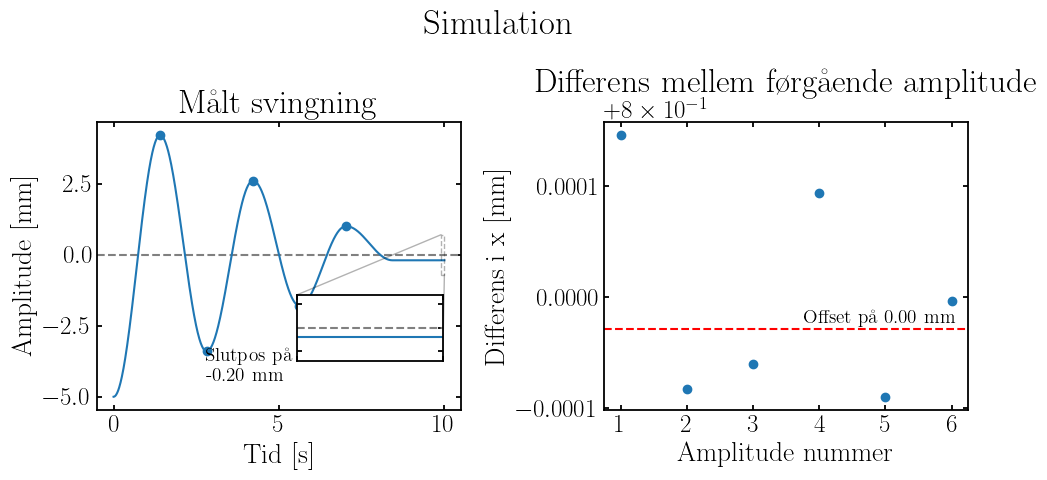
\includegraphics[width=0.8\linewidth,origin=c]{figures/Simulation.png}
    \caption{Simulering af differentalligningerne med $n_1=n_2=1$N, $k = 5$ N/mm, $\mu_s = \delta_s = 2$, og $\mu_k = \delta_k = 1$}
    \label{fig:simulering}
\end{figure}
Hvis vi løser differentialligningerne numerisk får vi resultatet på figur \ref{fig:simulering}, hvilket er i overrensstemmelse med de teoretiske resultater lige gennemgået. 
Specielt er dæmpningsfaktoren konstant (afvigelser kommer fra numerisk usikkerhed, alle værdierne er som man kan se inden for 0.0001 fra hinanden) og ligmed $\frac{2f_k}{k} = \frac{4 \text{N}}{5 \frac{\text{N}}{\text{mm}}} = 0.8 \text{mm}$.
Vi kan også beregne det teoretiske antal toppunkter (fra (7)). \[
    n_{\textup{slut}} = \left \lceil \frac{(5 \text{mm} - 0.8 \text{mm})}{0.8 \text{mm}} \right \rceil = 6 \text{mm}
\] 
Hvilket stemmer, og vi kan nu finde slutpunktet (fra (8))
\[
x(6) = (-1)^{6} (-5\text{mm} + 6 \cdot 0.8 \text{mm}) = 0.2 \text{mm}
\]
Hvilket igen stemmer overens med simuleringen.